\subsection{Introduction}
Dans cette partie nous allons voir comment l'attaque par analyse de consommation a été mise en place, c'est à dire comment fonctionne notre kit ChipWhisperer et utiliser pleinement ses fonctionnalités. Ceci comprend l'explication des firmwares, l'obtention et l'analyses des résultats obtenus.

\subsection{Installation de la ChipWhisperer (CW)}
Tout d'abord, nous avons pris en main le matériel, nous avons donc découvert les différentes cartes qui étaient à notre disposition dans le kit fournit.
Deuxièmement, nous avons branché physiquement la carte d'acquisition à un ordinateur via un port USB, c'est cette carte qui nous enverra la consommation de notre cible.

Nous nous sommes ensuite penché sur la connexion avec un ordinateur, afin de pouvoir communiquer avec la ChipWhisperer. Nous avons du chercher longuement afin de trouver comment nous connecter à cette carte via l'ordinateur. Pour ce faire, nous avons principalement consulté le wiki ChipWhisperer \cite{chip:rtd} et d'autres forums afin de trouver une solution. 
Nous avons donc commencé par installer les différents packages nécessaires pour utiliser la carte. Cette partie fut compliqué car le guide d'installation de la ChipWhisperer n'expliquait pas la marche à suivre pour nos OS respectifs. Cependant il était écrit qu'il était tout de même possible d'installer les paquets nécessaires au fonctionnement de la carte. Il a ainsi fallut installer chaque paquets un par un en trouvant le bon paquet disponible sur nos distributions. 

Ensuite nous avons installé JupyterNotebook, qui est un outil simple et accessible pour visualiser et organiser notre connexion et notre communication avec la carte. 
Il nous permettais de lancer chaque commande séparément et d'avoir le retour de la carte en conséquence.
Nous devions aussi utiliser un environnement python spécifique à l'aide de "pyenv" pour que notre JupyterNotebook fonctionne correctement.

\subsection{Fonctionnement de la ChipWhisperer (CW)}
Maintenant que notre environnement de travail est configuré et prêt à être utilisé, il va falloir communiquer avec la carte ! En utilisant le logiciel JupyterNotebook précédemment installé, nous avons pu suivre des ``notebooks'' d'introduction. À la fin de ces ``notebooks'', nous étions capable de flasher les firmwares d'introduction et de communiquer avec la carte en utilisant le protocole ``SimpleSerial''. En sommes, voici l'environnement que nous avons réussi à établir :

\begin{enumerate}
	\item Nous pouvons flasher un firmware sur la carte cible ;
	\item Nous pouvons nous connecter sur la carte d'acquisition en utilisant Python ;
	\item Nous pouvons communiquer avec la carte cible ;
	\item Nous pouvons déclencher des captures de consommations électrique.
\end{enumerate}

Une fois que nous avons complété les ``notebooks tutoriels'' fournit par le constructeur, nous allons essayer de faire une attaque très simple avec un firmware développé par un membre de la communauté.

\subsection{Premiers tests avec un projet développé par un membre de la communauté}
A ce niveau d'avancement du projet, nous sommes donc capable de flasher des firmwares déjà fait et de les utiliser en communiquant avec la carte cible à travers Python. Nous allons utiliser ces compétences pour essayé un projet développé par un membre de la communauté ChipWhisperer \cite{git:hell}, ce projet est une petite version du RSA avec les bons ``notebooks'' fournit et le firmware déjà créer. Nous avions juste à lancer le script python pour voir apparaitre cette trace de consommation électrique, cf Figure \ref{fig:hellmanconso}.
\begin{figure}[H]
	\centering
	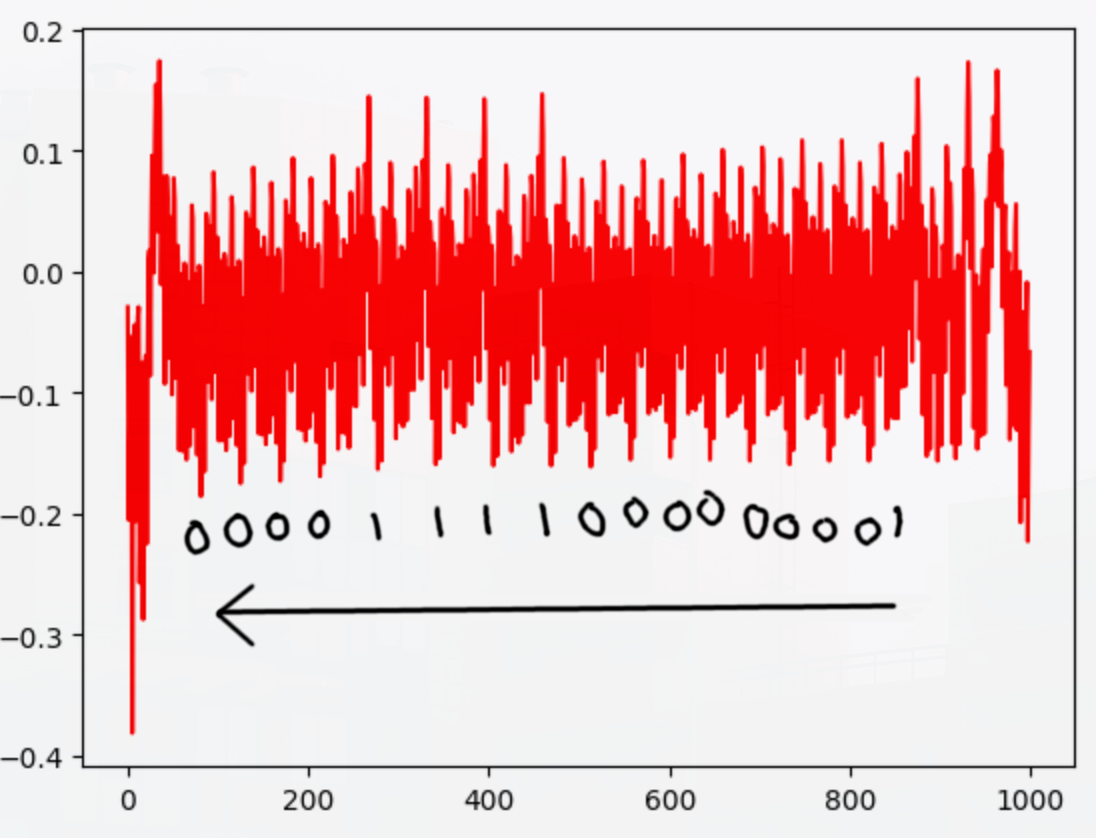
\includegraphics[width=\textwidth]{fig/hellman_conso.png}
	\caption{Schéma expliquant la commande de percussion - percussions actives}
	\label{fig:hellmanconso}
\end{figure}
Cette expérience à permis de nous mettre en confiance car nous nous sommes rendu compte qu'il est possible d'obtenir un résultat qui fonctionne avec notre matériel. En effet, nous pouvons lire aisément la clé sur la trace de consommation électrique, nous vous expliquerons plus en détail dans la suite de ce rapport la procédure à suivre. Nous allons donc pouvoir passer à l'implémentation de notre propre firmware.

\subsection{Conception de notre firmware}
À l'aide des algorithmes que nous vous avons expliqué et que nous avons implémenté en C dans la section précédente, il a été très facile pour nous de créer le fimware contenant le système RSA implémenté dedans. De plus avec l'expérience que nous avons acquise plus tôt, nous avons pu créer notre ``notebook'' facilement également. Nous avons donc tout qui est prêt pour passer à la cryptanalyse !

\subsection{Cryptanalyse}
Une fois que nous avions les traces de consommations, nous devons les exploiter afin de retrouver la clé privée utilisée et donc retrouver le message en clair. 
Les traces était sous la forme de tableaux sous python, il nous fallait donc utiliser la librairie matplotlib pour afficher les graphiques correspondants aux traces. 
Nous obtenions alors des traces comme celle ci-dessous:
\begin{figure}[H]
    \centering
    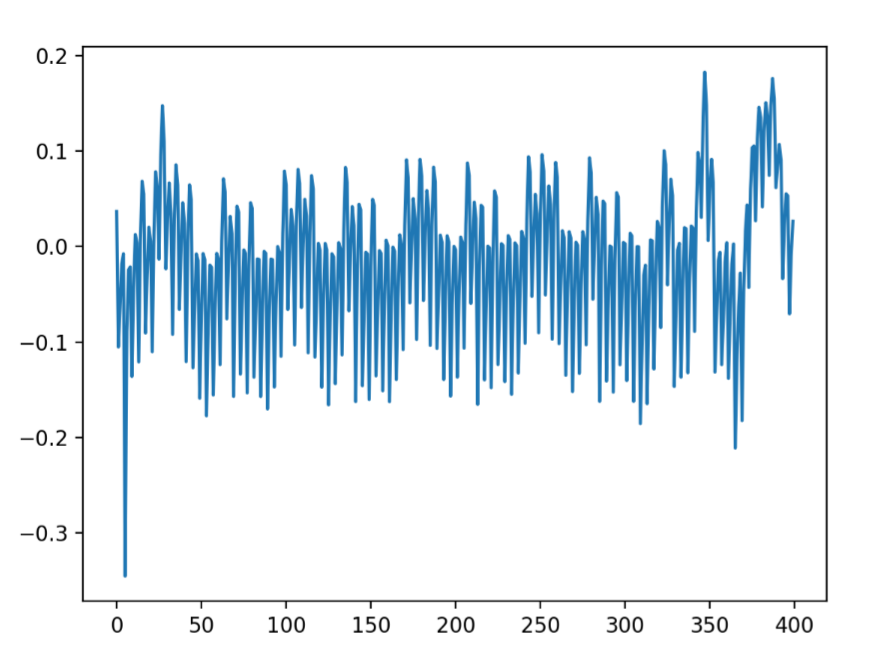
\includegraphics[width=0.8\textwidth]{fig/trace_brute.png}
    \caption{Trace brute de la consommation de courant}
    \label{fig:trace_brute}
\end{figure}
Dans ce cas nous avons utilisé la clé privé 11010101.
Cette trace n'est pas très lisible et nous avons donc utilisé une transformée de fourrier pour lisser la courbe. Après modification de la trace nous obtenons le graphique suivant:

\begin{figure}[H]
    \centering
    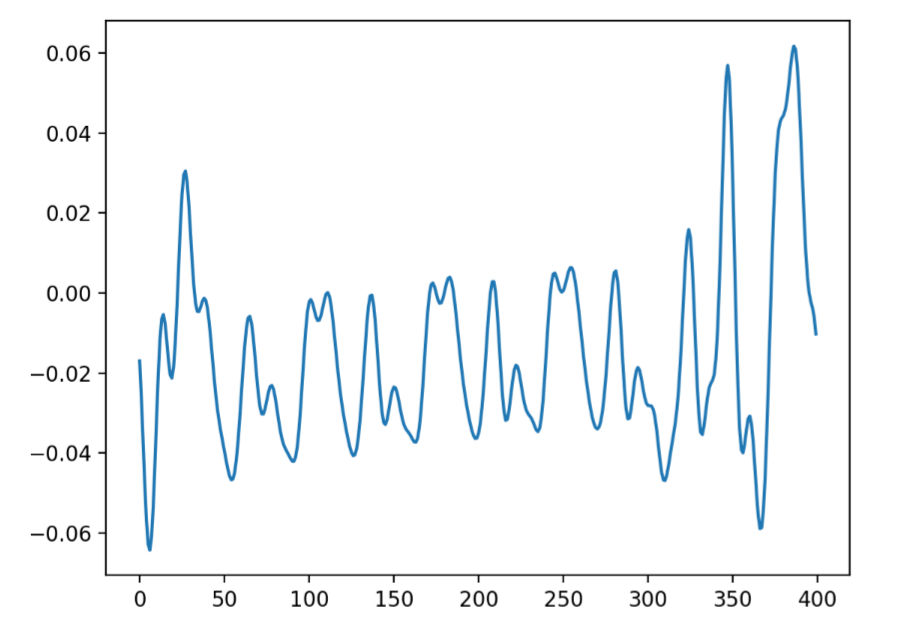
\includegraphics[width=0.8\textwidth]{fig/trace_tr.png}
    \caption{Trace lissée de la consommation de courant}
    \label{fig:trace_transforme}
\end{figure}
Nous voyons ainsi des patterns apparaître clairement sur le graphique.
l'algorithme d’exponentiation rapide se basant sur la représentation binaire de l'exposant les patterns apparaissant sur la trace correspondent aux 0 et 1 constituant l'exposant. La particularité de l’algorithme d'exponentiation rapide est qu'il parcours l'exposant du bit de poids faible au bit de poids fort et en fonction de la parité du bit actuel il va effectuer certaines opérations. Ainsi nous pouvons retrouver la clé utilisée pour déchiffrer le message.
Nous devons regarder les patterns présents en partant de la droite vers la gauche pour trouver la clé privé. Ayant au préalable testé l'attaque avec les clés 11111111 et 00000000 nous connaissions les correspondance entre les patterns et les chiffres binaires. Ainsi nous avons les correspondances suivantes :


\begin{minipage}[c]{0.45\textwidth}
\begin{figure}[H]
    \centering
    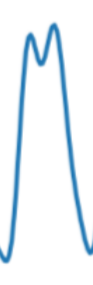
\includegraphics[width=0.1\textwidth]{fig/un.png}
    \caption{Pattern pour un 1}
    \label{fig:pat_un}
\end{figure}
\end{minipage}
\begin{minipage}[c]{0.45\textwidth}
\begin{figure}[H]
    \centering
    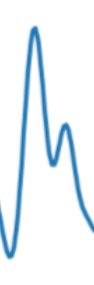
\includegraphics[width=0.1\textwidth]{fig/zero.png}
    \caption{Pattern pour un 0}
    \label{fig:pat_zero}
\end{figure}
\end{minipage}

\vspace{0.4 cm}
Nous pouvons ainsi retrouver la clé privé qui est 11010101 ce qui correspond bien à la clé utilisée.


\subsection{Automatisation}
La partie automatisation est assez importante car si nous devions déchiffrer sur 2048 bits, c'est à dire analyser une trace qui comprend 2048 pics de consommations différents, visuellement, la tache s'avérait longue et fastidieuse. L'automatisation d'une recherche de clés est donc essentielle et nous permet de gagner du temps d'analyse.
Pour automatiser la recherche de patterns nous voulions dans un premier temps utiliser une IA de classification binaire mais nous nous somme rendu compte que celle ci ne permet pas d'avoir une précision assez élevée. Ainsi sur 2048 bits, si 3 ou 4 bits sont faux sans qu'on sache lesquels nous ne pourront pas déchiffrer le message. Nous avons alors décidé d'utiliser un algorithme spécialisé dans la comparaison de pattern, l'algorithme de Pearson. Cette algorithme prend en entrée deux patterns et renvoie en sortie un coefficient de corrélation compris entre -1 et 1. A savoir que si le coefficient se tend vers -1 alors les deux patterns sont inversé, si le coefficient tend vers 0 alors les patterns n'ont rien en commun et enfin si le coefficient tend vers 1 les patterns sont très similaires. Nous avons ainsi utilisé un seuil de détection de 0,9 pour affirmer que deux patterns sont les mêmes. Nous avons ainsi développé une fonction qui parcours la trace et compare l'échantillon parcouru avec deux patterns correspondant au 1 et au 0.
Ainsi en utilisant cette fonction sur les traces vu précédemment, nous obtenons la clé 11010101.

\subsection{Validation de l'automatisation}
Afin de valider notre fonction d'automatisation, nous avons utilisé différentes clés générées aléatoirement et nous avons comparé ces clés avec le résultat de notre fonction. Le résultat est que sur 50 clés testés nous avons un taux de réussite de 100\% ce qui est très appréciable.